\section{\emph{rag}, a Ruby Autograder for ESaaS}

\subsection{Why Another Autograder?}

Given that 17 autograding systems and over 60 papers about them were
produced from 2006--2010 alone~\cite{ihantola-2010-autograding-survey},
why did we choose to build our own?
First, as the survey authors point
out, many existing systems' code
is not readily available or is tightly integrated to a particular Learning
Management System (LMS).  We needed to integrate with Coursera and
later OpenEdX, both of which were new and had not yet embraced
standards such as Learning Tools Interoperability\uf{imsglobal.org/lti}.
Unlike most previous 
systems, ours would need to work at ``cloud scale'' and respond to
workload spikes: the initial
offering of our MOOC in February 2012  
attracted over 50,000 learners, and we expected
that thousands of submissions would arrive bunched together close to the
submission deadline.  For the same reason, our graders needed to be
highly insulated from the LMS, so that students whose code accidentally
or deliberately damaged the autograder could not compromise other
information in the LMS.
Similarly, with a diverse and international group (less than
25\% of our MOOC learners were from the USA) with varied hardware,
software, and operating systems, autograding had to be ``zero
configuration,'' requiring no installation of software on learners' own
computers, and had to be trustworthy, in that the student
assignments were authoritatively graded on trusted servers rather than
having students self-report grades computed by their own computers.

Having chosen Ruby and Rails for their excellent testing and
code-grooming tools, our approach was to repurpose those same tools into
autograders that would give finer-grained feedback than human graders
using more detailed tests, and would be easier to repurpose than
those built for other languages.


\subsection{RSpecGrader}

\texttt{rag}\uf{github.com/saasbook/rag} 
is actually a collection of three different autograding
``engines'' based on three open source testing
tools.  The first of these is
RSpec, a unit-testing and
BDD/TDD framework descended from XUnit, but which exploits Ruby's
flexible syntax to embed a unit-testing DSL in Ruby that results in very
readable tests.  

\tbd{describe RSpecGrader, coverage, how to assign points to subparts,
how we can check internal structure of code/whether students used correct
abstractions, etc; maybe include snippet from an existing spec}

\tbd{Example of an RSpecGrader rubric file}

\subsection{FeatureGrader}

One of our assignments requires students to write integration-level
tests using Cucumber, which allows such tests to be formulated in
stylized plain text, as Figure~\ref{fig:cucumber} shows.

 Cucumber allows
integration-level tests or user stories~\cite{user-stories} to be
expressed in plain prose, using regular expressions to match each step
of such a test to a block of code that sets up preconditions (\texttt{Given}), stimulates
the system (\texttt{When}), or checks postconditions (\texttt{Then}) as
appropriate; our code blocks are in Ruby, but the Cucumber framework
itself is language-agnostic.  


Our autograder for this
style of assignment is inspired by mutation testing, a technique invented
by George Amman and Jeff 
Offutt~\cite{ammann-offutt-sw-testing} in which a
testing tool pseudo-randomly mutates the program under test to ensure
that some test fails as a result of these introduced errors.

%% Since a SaaS application is being tested, black-box integration tests
%% must stimulate the SaaS application in the same way that
%% a human being user a Web browser would.
%% Depending on the testing environment, Cucumber can do this in one of
%% three ways.  The first uses a built-in browser simulator that hooks
%% directly into 
%% the Rails application server, and thus can only be used
%% with application stacks that use this server and that do not rely on
%% JavaScript.  The second is using Webdriver (formerly 
%% Selenium) to control a real browser via a now-standard remote-control
%% API (cite Webremote).  The third, which we use, uses a Ruby library called
%% Mechanize\footnote{Based on the Perl library of the same name.} to
%% direct requests to an application deployed on  a remote server.  

\tbd{explanation of FeatureGrader basics}

\begin{figure}
  \begin{minipage}{0.45\textwidth}%
    \lstinputlisting{figs/cucumber_example.feature}%
  \end{minipage}%
  \begin{minipage}{0.5\textwidth}%
    \lstinputlisting[language=Ruby]{figs/cucumber_step_def_example.rb}%
  \end{minipage}%
  \caption{\label{fig:cucumber} Cucumber accepts integration tests 
    written in stylized prose (left) and uses regular expressions to map each
    step to a \emph{step definition} that sets up preconditions, exercises the app,
    or checks postconditions.  Step definitions 
    can stimulate a full-stack GUI-based web application in various
    ways, including remote-controlling a real browser with Webdriver
    (formerly Selenium) or using the Ruby Mechanize library to interact
    with a remote site.}
\end{figure}



\begin{figure}
  \begin{minipage}{0.45\textwidth}%
  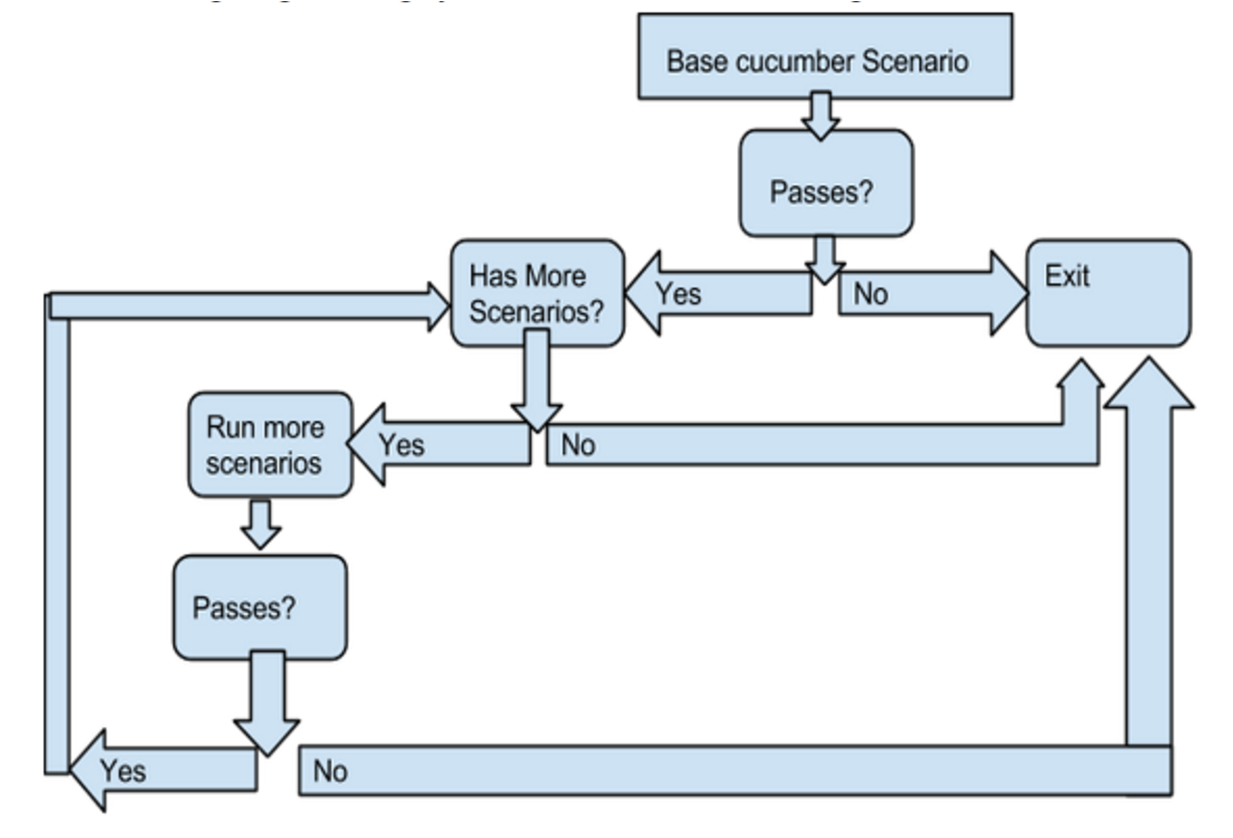
\includegraphics[width=\textwidth]{figs/feature_grader.pdf}%
  \end{minipage}%
  \begin{minipage}{0.55\textwidth}%
  \lstinputlisting{figs/feature_grader_example.yml}%
  \end{minipage}
  \caption{\label{fig:featuregrader}%
FeatureGrader workflow and example YAML file.  In this case if Step1-1 passes,
Step1-3 will be run next.  Earlier steps must be less restrictive than
later steps (if the earlier step fails, there should be no way that a later one could pass).
\texttt{failures} are the two student-provided Cucumber scenarios that \emph{should fail} when
run because of mutations (bugs) inserted in the app.
}
\end{figure}

\subsection{MechanizeGrader}

Surveys of recent
autograders~\cite{ihantola-2010-autograding-survey,douce-2005-autograding-survey} mentioned as
a ``future direction'' a grader that can assess full-stack or GUI apps.


Capybara~\uf{jnicklas.github.io/capybara}
provides a Ruby-embedded DSL for interacting with Web-based
applications.
One can trigger actions on a web page such as filling in form fields
or clicking a button, and use XPath~\cite{xpath} to examine the
response page delivered by the server.
Capybara actions can either run in the same process as the app being
tested, or when used in conjunction with the Mechanize
library~\footnote{\url{https://rubygems.org/gems/mechanize}; based on
  the older Perl library of the same name.}, can trigger these actions
against a remote application, allowing black-box testing.



Our MechanizeGrader achieves this by combining Capybara's embedded DSL
for interacting with a Web application with the Mechanize HTTP library
for interacting with and scraping a remote site.

\tbd{explain brefly how it works and how it's configured, how tests
  external app given just a URI, etc}

\tbd{cite AWAT as another example of GUI grader}


\begin{figure}
  \begin{tabular}{|p{0.15\textwidth}|p{0.15\textwidth}|p{0.7\textwidth}|}
 \hline
 \textbf{Grader} & \textbf{Based on} & \textbf{Student Assignment Type} \\
 \hline
 RSpecGrader &
 unit testing &
 Student submits one or more class files; black-box and ``intrusive''
 unit tests against functions and groups of functions are performed
 \\
 FeatureGrader &
 simplified mutation testing &
 Student submits integration tests written using Cucumber; bugs inserted
 in reference app attempt to trigger test failures to check test suite
 completeness and test fragility
 \\
 MechanizeGrader & 
 staging-like integration testing &
 Student deploys full-stack app to public cloud; ``black box'' tests
 stimulate remote server and parse/analyze output, including execution
 of JavaScript if needed
 \\
 \hline
\end{tabular}

  \caption{\label{fig:grader_summary} Summary of the autograder
    engines: grader types, types of assignments they grade, and
    how students submit work}
\end{figure}


